% Figure 2 of the methods paper, the router size map, written by
% scripts/paper-methods-figure.py from the same ROUTERS as
% site/public/paper/methods/figure-2.svg. Do not edit: run the script again.
\definecolor{paperfigblue}{HTML}{0284C7}
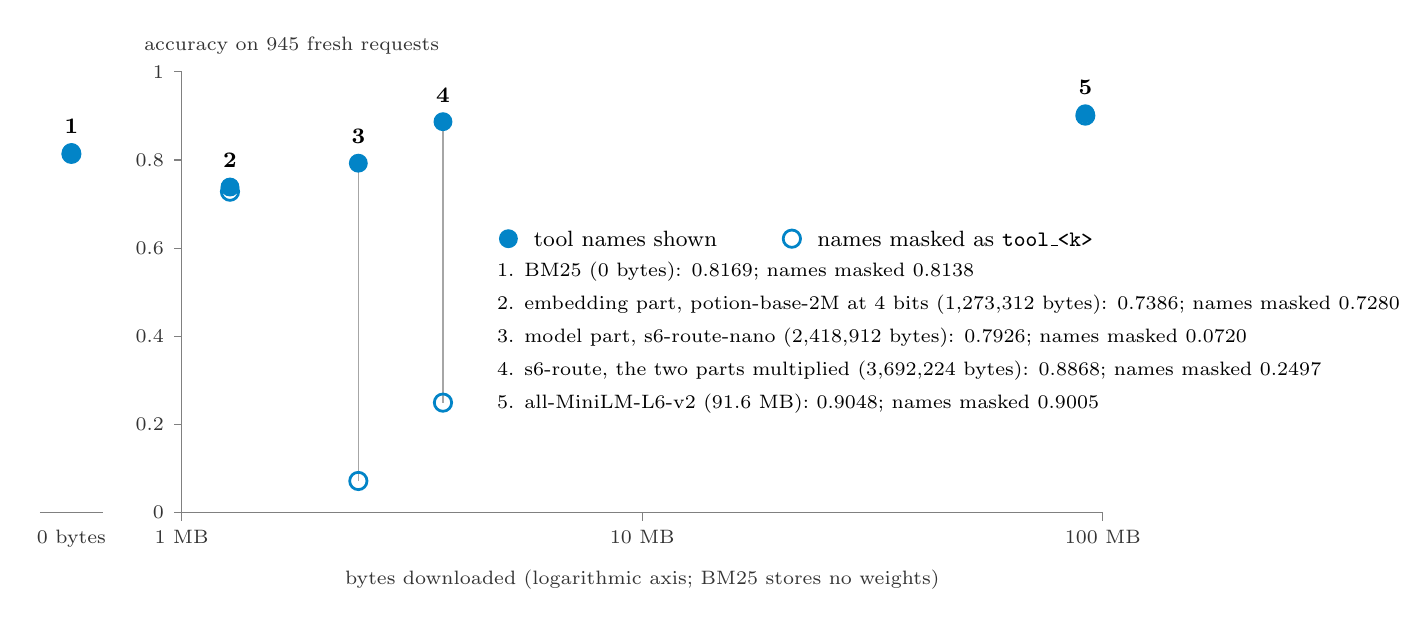
\begin{tikzpicture}[x=1cm,y=1cm,font=\footnotesize]
\draw[black!50] (2.9,1.2) -- (14.6,1.2);
\draw[black!50] (1.10,1.2) -- (1.90,1.2);
\draw[black!50] (2.9,1.2) -- (2.9,6.8);
\draw[black!50] (2.900,1.2) -- (2.900,1.10) node[below,text=black!80,font=\scriptsize] {1 MB};
\draw[black!50] (8.750,1.2) -- (8.750,1.10) node[below,text=black!80,font=\scriptsize] {10 MB};
\draw[black!50] (14.600,1.2) -- (14.600,1.10) node[below,text=black!80,font=\scriptsize] {100 MB};
\node[below,text=black!80,font=\scriptsize] at (1.5,1.10) {0 bytes};
\node[text=black!80,font=\scriptsize] at (8.75,0.35) {bytes downloaded (logarithmic axis; BM25 stores no weights)};
\draw[black!50] (2.9,1.200) -- (2.80,1.200) node[left,text=black!80,font=\scriptsize] {0};
\draw[black!50] (2.9,2.320) -- (2.80,2.320) node[left,text=black!80,font=\scriptsize] {0.2};
\draw[black!50] (2.9,3.440) -- (2.80,3.440) node[left,text=black!80,font=\scriptsize] {0.4};
\draw[black!50] (2.9,4.560) -- (2.80,4.560) node[left,text=black!80,font=\scriptsize] {0.6};
\draw[black!50] (2.9,5.680) -- (2.80,5.680) node[left,text=black!80,font=\scriptsize] {0.8};
\draw[black!50] (2.9,6.800) -- (2.80,6.800) node[left,text=black!80,font=\scriptsize] {1};
\node[anchor=south west,text=black!80,font=\scriptsize] at (2.30,6.90) {accuracy on 945 fresh requests};
\draw[black!35,line width=0.6pt] (1.500,5.775) -- (1.500,5.757);
\draw[paperfigblue,line width=1pt] (1.500,5.757) circle (0.11);
\fill[paperfigblue] (1.500,5.775) circle (0.12);
\node[anchor=south,font=\footnotesize\bfseries] at (1.500,5.895) {1};
\draw[black!35,line width=0.6pt] (3.514,5.336) -- (3.514,5.277);
\draw[paperfigblue,line width=1pt] (3.514,5.277) circle (0.11);
\fill[paperfigblue] (3.514,5.336) circle (0.12);
\node[anchor=south,font=\footnotesize\bfseries] at (3.514,5.456) {2};
\draw[black!35,line width=0.6pt] (5.144,5.639) -- (5.144,1.603);
\draw[paperfigblue,line width=1pt] (5.144,1.603) circle (0.11);
\fill[paperfigblue] (5.144,5.639) circle (0.12);
\node[anchor=south,font=\footnotesize\bfseries] at (5.144,5.759) {3};
\draw[black!35,line width=0.6pt] (6.219,6.166) -- (6.219,2.598);
\draw[paperfigblue,line width=1pt] (6.219,2.598) circle (0.11);
\fill[paperfigblue] (6.219,6.166) circle (0.12);
\node[anchor=south,font=\footnotesize\bfseries] at (6.219,6.286) {4};
\draw[black!35,line width=0.6pt] (14.377,6.267) -- (14.377,6.243);
\draw[paperfigblue,line width=1pt] (14.377,6.243) circle (0.11);
\fill[paperfigblue] (14.377,6.267) circle (0.12);
\node[anchor=south,font=\footnotesize\bfseries] at (14.377,6.387) {5};
\fill[paperfigblue] (7.05,4.68) circle (0.12);
\node[anchor=west] at (7.25,4.68) {tool names shown};
\draw[paperfigblue,line width=1pt] (10.65,4.68) circle (0.11);
\node[anchor=west] at (10.85,4.68) {names masked as \texttt{tool\_<k>}};
\node[anchor=west,inner sep=0pt,font=\scriptsize] at (6.90,4.26) {1. BM25 (0 bytes): 0.8169; names masked 0.8138};
\node[anchor=west,inner sep=0pt,font=\scriptsize] at (6.90,3.84) {2. embedding part, potion-base-2M at 4 bits (1,273,312 bytes): 0.7386; names masked 0.7280};
\node[anchor=west,inner sep=0pt,font=\scriptsize] at (6.90,3.42) {3. model part, s6-route-nano (2,418,912 bytes): 0.7926; names masked 0.0720};
\node[anchor=west,inner sep=0pt,font=\scriptsize] at (6.90,3.00) {4. s6-route, the two parts multiplied (3,692,224 bytes): 0.8868; names masked 0.2497};
\node[anchor=west,inner sep=0pt,font=\scriptsize] at (6.90,2.58) {5. all-MiniLM-L6-v2 (91.6 MB): 0.9048; names masked 0.9005};
\end{tikzpicture}
